\documentclass{article}

\usepackage[english]{babel}
\usepackage[letterpaper,top=2cm,bottom=2cm,left=3cm,right=3cm,marginparwidth=1.75cm]{geometry}

% Useful packages
\usepackage{amsmath}
\usepackage{csvsimple}
\usepackage{graphicx}
\usepackage{verbatim}
\usepackage{listings}
\usepackage[colorlinks=true, allcolors=blue]{hyperref}
\usepackage[utf8]{inputenc}
\lstdefinestyle{Rstyle}{
    language=R,
    basicstyle=\small\ttfamily\color{black},
    numbers=left,
    numberstyle=\tiny\color{black},
    breaklines=true,
    stepnumber=1,
    numbersep=10pt,
    backgroundcolor=\color{white},
    showspaces=false,
    showstringspaces=false,
    showtabs=false,
    frame=single,
    tabsize=1,
    captionpos=b,
    breakatwhitespace=false,
    title=\lstname,
}

\title{Outliers Learn}

\author{
  \normalsize Author: Andr
  \normalsize Tutor: Juan Jos
  \normalsize Degree: Degree in Informatics Engineering
}

\date{December 2023}

\usepackage{Sweave}
\begin{document}
\input{OutliersLearn-concordance}
\maketitle

\begin{abstract}
Your abstract.
\end{abstract}

\section{Introduction}
In the dynamic landscape of data analytics, identifying outliers is critical. As The New York Times describes, outliers, "a statistical observation that is markedly different in value from the others of the sample" \label{intro:nytimes}[1].
Detecting this anomalies can be a huge challenge at first sight but, thanks to past years investigations, data scientist can benefit from various algorithms that can solve this issue.
To address this challenge, we are delighted to introduce the "OutliersLearn" package, a toolkit dedicated to learning outlier detection in R.

\section{About outliers}
As it was mentioned earlier, we can describe outliers as observations that has an abnormal distance from other values in a random sample from a population \label{outliers:definition}[2]. But, are all outliers the same? Do they have to be treated the same way? Do they have any type of effect on the algorithms used in data analysis, deep-learning, etc.?
To understand outliers better and to solve this question, they can classified in two main types:
\begin{itemize}
    \item Wrong data, coming from measurement errors, which must be eliminated because they will lead to data analysis with erroneous conclusions. This type of outliers are treated in the pre-processing stage (data cleaning) using various techniques that will lead to different results on the final dataset.
    \item Correct data, with a lot of significance, that deviates from the normal and must be analyzed very carefully because it can lead to important findings.
\end{itemize}

It's extremely obvious that this two types of outliers must not be treated the same. The first one (wrong data) includes "human errors" (e.g. misspelling a value), distorted measurements, etc. The second one are genuine values that really have an impact on the data (e.g. The Wall Street Crash of 1929), this type of data must be counted in the dataset because it's not an error, it's a significant value.
Going back to the questions proposed earlier, outliers do have effect on the data. This can be for worse of for better, depending on the type of outlier (e.g. if the dataset used for a technique/algorithm includes wrong values, this can lead to worse results in the designated study).

This is an example of the effect of an outlier in a linear regression algorithm result:
\begin{figure}
    \centering
    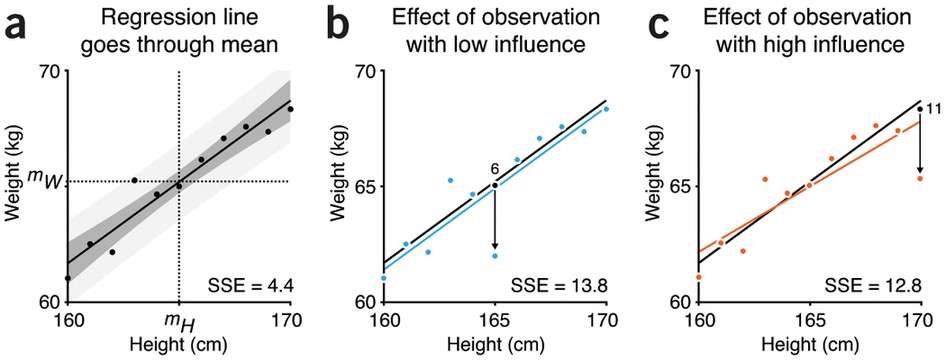
\includegraphics[width=0.6\textwidth]{./images/outlierEffectExample.jpg}
    \caption{Outliers effect linear regression}
    Image source \label{fig:outliers_effect}[3]
\end{figure}
As we can see, including an outlier on a linear regression algorithm has effect on the result. If this outlier is wrong data, it will lead to worse predictions due to the fact that the regression line is modified by that/those value/s. If the outlier is a true value, then the predictions made by the regression line will take into account the anomaly and it will lead to more precise predictions.

Studies to identify anomalous events or outliers seek to find and categorize as outliers those events that are very different from the rest of those that make up the studied sample. To give a measure of how anomalous an event is we use the outlier score (its definition depends on the technique used). The degree of outlier is set arbitrarily by the data analyst taking into account the study being carried out.
The classification of outlier identification techniques depends on the technique used in the analysis:
\begin{itemize}
    \item Based on proximity: they look for events that are very separated from the rest of the events, they are based on the definition of distances (e.g. KNN)
    \item Based on density: they look for events that are in a spatial area in which there is a lower density than the observed average (e.g. LOF).
    \item Cluster-based: They apply to previously clustered events. (e.g BDSCAN clustering algorithm)
    \item Statistic methods can be classified in:
    \begin{itemize}
        \item Organization (box and whiskers)
        \item Dispersion
        \item Regression
    \end{itemize}
\end{itemize}

\section{Objectives and field of application}
This project has as field of study the study and application of outlier detection algorithms as a learning R package as well as the implementation of those algorithms. The most used algorithms in outlier detection will be studied, as well as the most modern ones (developing them in a package dedicated to learning outlier detection).
The main objective that is chased by developing this R package is to provide an R package that can be used in the academic and professional fields to learn data anomaly detection algorithms in a simple and intuitive way.
The package will allow users to gain hands-on experience in outlier detection. By providing a comprehensive learning environment, this project seeks to bridge the gap between theoretical knowledge and practical implementation. By using this R package, people will improve their knowledge of outlier detection algorithms, which will contribute to the advancement of data analysis and decision-making processes.

\section{Work description}
As it has been mentioned earlier, the main task is to develop an R package that helps on the learning process of outlier detection algorithms. To archive this, the first part of the project will explain this algorithms more deeply (using a more theoretical explanation).
The second part will be centered on the development of the package in R (programming the functions/algorithms that have been explained on the previous part). This package will include tools that can be used to detect algorithms in a learning environment (to understand how the algorithms work from a more practical point of view).
Finally there will be included some examples, interesting cases and how outliers affect different algorithms depending on the situation.

\section{OutliersLearn R Package}
\subsection{Introduction}
This R package is dedicated to learning how determinate algorithms work. It can be installed via CRAN or GitHub as it will be mentioned in the \ref{outliers:install} section (How to install). This package has been fully developed in R and the code to each algorithm can be found in the \ref{outliers:annex} section (Annex). This section will then be dedicated to the explanation of each algorithm, use cases, calling the algorithm examples and execution examples with an explanation of the results.

\subsection{Implemented algorithms}
There are lots of algorithms that could have been implemented. It has been selected a subset of algorithms based on their utility, common use and importance. These algorithms are the nex ones:
\begin{itemize}
    \item Box and Whiskers Method
    \item KNN
    \item LOF
    \item Mahalanobis Method
    \item Standard Deviation and Mean method
    \item DBSCAN
\end{itemize}
It is also important to highlight the fact that it has been developed more functions (auxiliary functions) that are necessary for this algorithms. They will be explained later on but this are the auxiliary functions developed:
\begin{itemize}
    \item Euclidean distance
    \item Mahalanobis distance
    \item Manhattan distance
    \item Transform to vector
    \item Quantiles calculation function
\end{itemize}

\subsection{Box and Whiskers Method}
This algorithm is based on the calculation of quartiles and value limits. It can be resumed in 4 main steps:
\begin{enumerate}
    \item Determine the degree of outlier or distance at which an event is considered an outlier. This "parameter" is determined arbitrarily so it's the decision of the user the value that it has. It directly affects the algorithm as it will be explained later.
    \item Sort the data and obtain the quartiles
    \item Calculate the interval limits for outliers using the next equation:
    \begin{center}
    \(
    (Q_1 - d \cdot (Q_3 - Q_1), \: Q_3 + d \cdot (Q_3 - Q_1))
    \)
    \end{center}
    \(Q_1\) is the 1st quartile, \(Q_3\) is the third quartile and \(d\) is the degree of outlier or distance at which an event is considered an outlier.
\end{enumerate}
As it can be seen, the value of \(d\) directly affects the results of the algorithm. This value is independent from the "scale" of the values of the dataset. When incrementing the value of \(d\), the range of the limits is bigger and more data will be "inside" those limits so there will be less outliers.
The figure \ref{fig:box&whiskerslimitsexample} is a graphical example of the limits obtained with this algorithm. As it can be seen, the low limit is calculated with the formula explained before. Same happens with the top limit.
\begin{figure}
    \centering
    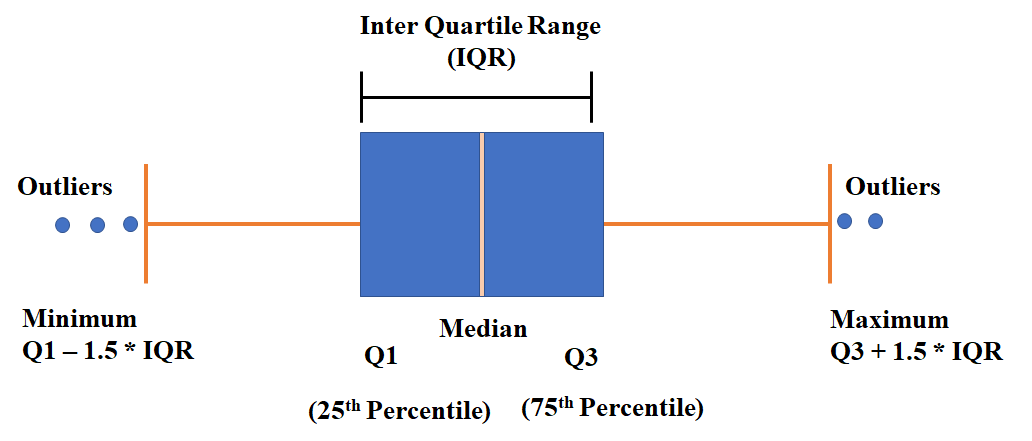
\includegraphics[width=0.6\textwidth]{./images/BoxAndWhiskersExample.png}
    \caption{Box and whiskers example}
    Image source \label{fig:box&whiskerslimitsexample}[4]
\end{figure}

Every single value that is not "inside" this limits is considered an outlier. To get all the outliers of the dataset is as easy as checking if every single value/event is or not inside the limits calculated before.
The pros and cons will be discussed later on but it's easy to see that this algorithm is extremely easy to implement. It's crucial to highlight that the implementation has been done for 1D vectors. The algorithm for multidimensional vectors should be the same (applied over one of the columns of the dataset), as it can be deduced, this is not a good method to obtain outliers out of a multidimensional dataset (there is always some exceptions). That's why it has been implemented only over 1D arrays/vectors.

\subsubsection{Auxiliary functions used}
The main function that has been implemented for the "Box and Whiskers Algorithm" is named "quantile\_outliersLearn". This function is dedicated to calculate the value of the quantile indicated over the input data. The function itself looks like this:
\begin{center}
    \begin{lstlisting}[style=RStyle, caption=quantile\_outliersLearn function code]
quantile_outliersLearn <- function(data,v){
  data = transform_to_vector(data);
    data = sort(data);
    nc = length(data)*v;
    if (is.integer(nc)) {
            x = (data[nc] + data[nc+1])/2;
    } else {
            x = data[floor(nc)+1];
    }
    return(x)
}
    \end{lstlisting}
\end{center}
As it has been said before, this function calculates the value of the quantile indicated in the input dataset. Pseudocode can be used to understand better how functions work. This is the pseudocode to the quantile\_outliersLearn() function:
\begin{enumerate}
    \item Sort the input data
    \item Obtain the nc value means n*quantile. This is, the number of elements in the input dataset times the value of the quantile (v). The value of the quantile must be between 0 and 1. This value (v) indicates the quantile that it's desired to calculate. For example, for the first and third quartiles the values are 0.25 and 0.75. The value nc will be used to get the elements at that position so it's a "pointer" or an index to a determined position of the input dataset.
    \item The last step is to calculate the value of the quantile. There are 2 main scenarios:
    \begin{enumerate}
        \item If the value of nc is a whole number, the value of the quantile is calculated with this equation:
        \begin{center}
        \(
        x = \frac{{\text{Data in position } nc + \text{Data in position } (nc+1)}}{2}
        \)
        \end{center}
        \item If the value of nc is not a whole number the value of the quantile is calculated with this equation:
        \begin{center}
        \(
        x = \text{Data in position } nc \text{ rounded down } + 1
        \)
        \end{center}
        The +1 is for the position, not for the value (valid for both cases)
    \end{enumerate}
\end{enumerate}
Here is an example of execution of this function:
\begin{Schunk}
\begin{Sinput}
> source("./code/quantile_outliersLearn.R")
> source("./code/transform_to_vector.R")
> (data = c(1,2,3,4,1,6,10,20))
\end{Sinput}
\begin{Soutput}
[1]  1  2  3  4  1  6 10 20
\end{Soutput}
\begin{Sinput}
> (q1 = quantile_outliersLearn(data, 0.25))
\end{Sinput}
\begin{Soutput}
[1] 2
\end{Soutput}
\begin{Sinput}
> (q2 = quantile_outliersLearn(data, 0.5))
\end{Sinput}
\begin{Soutput}
[1] 4
\end{Soutput}
\begin{Sinput}
> (q3 = quantile_outliersLearn(data, 0.75))
\end{Sinput}
\begin{Soutput}
[1] 10
\end{Soutput}
\begin{Sinput}
> (q = quantile_outliersLearn(c(12,2,3,4,1,13), 0.60))
\end{Sinput}
\begin{Soutput}
[1] 4
\end{Soutput}
\end{Schunk}
As it can be seen, this function also uses the transform\_to\_vector() function. This function is dedicated to the transformation of any type of data into a vector. The code is this but it won't be explained in detail due to the fact that is not that relevant to the "theory" behind the algorithm. It's more of a normalization function for data.
\begin{lstlisting}[style=RStyle, caption="transform\_to\_vector code"]
transform_to_vector <- function(data) {
  if (is.numeric(data)) {
    return(data)
  } else if (is.character(data)) {
    return(as.character(data))
  } else if (is.logical(data)) {
    return(as.numeric(data))
  } else if (is.factor(data)) {
    return(as.character(data))
  } else if (is.integer(data)) {
    return(as.numeric(data))
  } else if (is.complex(data)) {
    return(Mod(data))
  } else if (is.list(data)) {
    return(unlist(data))
  } else if (is.data.frame(data)) {
    return(as.vector(data))
  } else if (is.matrix(data)) {
    return(as.vector(data))
  } else if (is.array(data)) {
    return(as.vector(data))
  } else if (is.table(data)) {
    return(as.vector(data))
  } else if (is.environment(data)) {
    return(ls(data))
  } else if (isS4(data)) {
    return(unclass(data))
  } else if (is.raw(data)) {
    return(as.numeric(data))
  } else {
    warning("Data type not recognized. Returning as is.")
    return(data)
  }
}
\end{lstlisting}
It checks every single data type that can be converted to vector and converts it to that type.

\subsubsection{Pros and cons of this algorithm}
(TODO)
\subsubsection{Algorithm parameters \& Output}
This section will be dedicated to the explanation of the parameters (input \& output) of the box and whiskers algorithm implemented in the OutliersLearn R package.
\paragraph{Input parameters}
The input parameters to the function are:
\begin{itemize}
    \item data: Input data
    \item d: Degree of outlier or distance at which an event is considered an outlier
    \item tutorialMode: if TRUE the tutorial mode is activated
\end{itemize}
As it can be seen, we have the parameters of the algorithm itself and then an extra one that depending on the value of it (TRUE or FALSE), the process will show all the steps and an explanation to it (tutorial mode enabled if TRUE) or not (tutorial mode disabled if FALSE).
Here are some examples of parameters of this function so it can be better understood:
\begin{lstlisting}[style=RStyle, caption="Examples of parameters for the boxandwhiskers function]
#First example of input parameters:
inputData = t(matrix(c(3,2,3.5,12,4.7,4.1,5.2,4.9,7.1,6.1,6.2,5.2,14,5.3),2,7,dimnames=list(c("r","d"))))
inputData = data.frame(inputData)
d = 2
tutorialMode = TRUE
#Second example of input parameters:
inputData = c(1,2,3,4,1,23,4)
d = 3
tutorialMode = FALSE
\end{lstlisting}
\paragraph{Output of the algorithm}
The output of this algorithm includes a "text" output indicating the outliers obtained as well as a graphical output. Due to the nature of the R package is included in, the output is shown in the R console (for the text output) and in the corresponding Plot section (for the visual output). The function itself does not return anything (does not matter if the tutorial mode is enabled or not).
\subsubsection{How to use this algorithm \& Examples of execution}
\label{outliers:howtousebandw}
As it has been mentioned earlier, the input parameters are: data, d and tutorialMode. This are some examples of calling the function boxandwhiskers() in R. This section is dedicated just to show how to call this function and some results obtained. Section \ref{outliers:explanationexecutionbandw} has a full explained execution of the algorithm showing how it works and an explanation of the results. Now the tutorialMode will be set to FALSE because of this. Here are 2 examples of code execution:
\begin{Schunk}
\begin{Sinput}
> source("./code/boxandwhiskers.R")
> inputData = t(matrix(c(3,2,3.5,12,4.7,4.1,5.2,4.9,7.1,6.1,6.2,5.2,14,5.3),2,7,dimnames=list(c("r","d"))))
> inputData = data.frame(inputData)
> boxandwhiskers(inputData,2,FALSE)
\end{Sinput}
\begin{Soutput}
[1] "Obtained limits: "
  d3   r6 
-0.1 10.4 
[1] "The value in position 7 with value 14.000 has been detected as an outlier"
[1] "It was detected as an outlier because it's value is higher than the top limit 10.400"
[1] "--------------------------------------------------------------------------------------------"
[1] "The value in position 9 with value 12.000 has been detected as an outlier"
[1] "It was detected as an outlier because it's value is higher than the top limit 10.400"
[1] "--------------------------------------------------------------------------------------------"
\end{Soutput}
\end{Schunk}
Another example:
\begin{Schunk}
\begin{Sinput}
> boxandwhiskers(c(1,2,3,4,1,23,4),2,FALSE)
\end{Sinput}
\begin{Soutput}
[1] "Obtained limits: "
[1] -5 10
[1] "The value in position 6 with value 23.000 has been detected as an outlier"
[1] "It was detected as an outlier because it's value is higher than the top limit 10.000"
[1] "--------------------------------------------------------------------------------------------"
\end{Soutput}
\end{Schunk}
\subsubsection{Example of execution of this algorithm with result explanation}
\label{outliers:explanationexecutionbandw}
Here is the execution of the example shown in the section \ref{outliers:howtousebandw} but now with the tutorial mode activated (with the full explanation)
\begin{Schunk}
\begin{Sinput}
> boxandwhiskers(c(1,2,3,4,1,23,4),2,TRUE)